\documentclass[11pt,a4paper]{article}
\usepackage[utf8]{inputenc}
\usepackage[T1]{fontenc}
\usepackage{lmodern}
\usepackage[brazil]{babel}
\usepackage[margin=1in]{geometry}
\usepackage{authblk}
\usepackage{amsmath,amssymb,amsfonts}
\usepackage{graphicx}
\usepackage{booktabs}
\usepackage{xcolor}
\usepackage{hyperref}
\usepackage{cite}
\usepackage{microtype}
\usepackage{fancyhdr}
\usepackage{enumitem}
\hypersetup{colorlinks=true,linkcolor=blue!50!black,citecolor=blue!50!black,urlcolor=blue!50!black,pdftitle={Tokenaholics: O Novo Vício Silencioso da Era da Inteligência Artificial},pdfauthor={Murillo Edson de Carvalho Souza}}
\pagestyle{fancy}
\fancyhf{}
\fancyhead[L]{\small Tokenaholics: autonomia e dependência na era da IA}
\fancyhead[R]{\small\thepage}
\setlength{\headheight}{14pt}
\renewcommand{\headrulewidth}{0.4pt}
\setlist{itemsep=3pt,topsep=5pt}
\emergencystretch=2em
\clubpenalty=10000
\widowpenalty=10000
\displaywidowpenalty=10000
\author[1]{\textbf{Murillo Edson de Carvalho Souza}}
\affil[1]{Universidade de Brasília (UnB)\\Departamento de Ciências da Computação}
\date{}
\begin{document}
\title{\textbf{Tokenaholics: O Novo Vício Silencioso da Era da Inteligência Artificial}\\[0.5em]\large Uma análise sociotécnica com dados públicos, aprendizagem de máquina e cenários de consumo}
\maketitle
\begin{abstract}
A expansão da inteligência artificial generativa torna necessário distinguir consumo computacional, adoção e dependência problemática. Propõe-se \textit{Tokenaholics} como conceito exploratório, sem equivalência diagnóstica, e combina-se revisão crítica interdisciplinar com análise secundária de agregados públicos de 2025 e 2026. São examinados perfis de uso da Anthropic por país e grupo ocupacional, participações diárias de tokens e gastos da Vercel e indicadores do GitHub. O K-means em cinco variáveis seleciona uma partição em dois grupos entre 121 países, com separação limitada (silhouette de 0,308). O cruzamento GitHub--Anthropic reúne oito dos dez países da tabela GitHub. Computação e matemática têm participação publicada de 23,80\% no chat e 28,17\% na API em maio de 2026; essas medidas preservam os denominadores de cada canal. A avaliação temporal de Ridge e três baselines não sustenta superioridade preditiva estável. Cenários orçamentários para 2027 combinam quantidade de tokens e preço efetivo sob composição constante. Os achados descrevem heterogeneidade geográfica, diferenças entre canais e distribuições distintas de tokens e despesa. Esses resultados caracterizam o contexto sociotécnico, sem operacionalizar ou validar Tokenaholics, estimar prevalência de dependência ou identificar causalidade. A contribuição para a computação é articular uma definição conceitual delimitada a procedimentos reproduzíveis de análise e a uma agenda futura de avaliação de regulação, verificação e prejuízo funcional.
\end{abstract}
\noindent\textbf{Palavras-chave:} inteligência artificial generativa; modelos de linguagem; confiança excessiva; autonomia cognitiva; engenharia de software; uso problemático de IA.

\section{Introdução}
Uma resposta aparece antes que o problema esteja inteiramente formulado. Um trecho de código funciona antes que sua lógica tenha sido compreendida. Uma segunda consulta oferece a confirmação que a primeira não forneceu. Essas situações, aqui utilizadas como exemplos hipotéticos, ajudam a formular uma questão: quando a assistência computacional amplia a capacidade de agir e quando passa a substituir as condições necessárias para julgar o próprio trabalho?

O problema interessa particularmente à ciência da computação. Ferramentas generativas participam da produção de código, da documentação, dos testes e da análise de requisitos. A revisão de Fan et al. \cite{fan} situa essas aplicações em diferentes atividades de engenharia de software e destaca desafios de correção e verificação. A mudança relevante não se limita ao tamanho dos modelos: envolve quem formula objetivos, como se testa uma resposta e quem assume responsabilidade pelo resultado.

Neste artigo, propõe-se \textit{Tokenaholics} como denominação exploratória para investigar uma relação de dependência operacional e cognitiva potencialmente problemática em ambientes mediados por IA generativa. A unidade lexical remete aos tokens processados pelos modelos e evoca, deliberadamente, a linguagem cultural do excesso. A proposta pertence ao autor deste manuscrito; isso não estabelece prioridade mundial da palavra, exclusividade de uso ou a descoberta de uma nova doença. A contribuição pretendida está na definição delimitada e na agenda de investigação associada ao termo.

A expressão ``novo vício silencioso'' exige cuidado. ``Novo'' designa a configuração técnica examinada, e não a inexistência de antecedentes de dependência tecnológica. ``Silencioso'' indica a possibilidade de prejuízos pouco visíveis em métricas de entrega, hipótese a testar. ``Vício'' funciona como provocação do título. No corpo analítico, empregam-se uso problemático, delegação persistente e confiança excessiva, sem supor equivalência entre essas categorias.

A pergunta orientadora é: \textit{como delimitar uma proposta sobre delegação problemática à IA generativa e caracterizar seu contexto de uso sem confundir intensidade computacional, adoção e dependência clínica?} O objetivo geral é articular uma definição conceitual informada pela literatura a uma caracterização empírica de práticas agregadas de uso. Especificamente, busca-se: (i) distinguir mecanismos computacionais e conceitos de dependência; (ii) descrever perfis nacionais, composições ocupacionais e associações ecológicas entre indicadores; (iii) comparar participações de tokens e gasto; (iv) avaliar previsões locais de participação e cenários orçamentários; e (v) delimitar quais evidências futuras seriam necessárias para investigar uso problemático.

O estudo utiliza análise empírica secundária de agregados, sem recrutamento de participantes ou escala clínica. Sua estrutura reúne dois componentes complementares: a literatura fundamenta a definição e suas dimensões propostas; os dados descrevem o contexto de uso e os limites da mensuração computacional. As unidades empíricas são países, grupos ocupacionais e séries de participação em plataforma. Não há medidas individuais de regulação, compreensão ou prejuízo funcional; portanto, os resultados agregados não constituem teste da ocorrência de Tokenaholics.

\section{Método: revisão crítica e análise secundária}
\subsection{Desenho, recorte e seleção}
O desenho combina revisão narrativa crítica com busca dirigida e análise exploratória de dados secundários. O núcleo temático reúne doze trabalhos científicos com publicação formal ou versão identificada entre 2022 e 2026. A bibliografia contém ainda dezessete referências complementares, incluindo dois preprints empíricos, relatórios, bases e documentação técnica, totalizando 29 entradas. O ano de publicação não é tomado como ano de medição de cada indicador. Não se pretende cobertura exaustiva, revisão sistemática ou metanálise.

Foram utilizadas buscas na web acadêmica, páginas de editoras e repositórios de autores, com prioridade para registros no IEEE Xplore. Consultaram-se expressões em inglês como \textit{large language models software engineering}, \textit{Copilot security}, \textit{AI overreliance}, \textit{critical thinking generative AI}, \textit{problematic artificial intelligence use}, \textit{anthropological AI} e \textit{artificial intelligence and work}. Crossref foi empregado para confrontar DOI, autoria, título, veículo e datas; repositórios institucionais e arXiv forneceram versões acessíveis. Resultados de busca serviram à descoberta, e não substituíram a consulta ao conteúdo das fontes incluídas.

Incluíram-se trabalhos com contribuição direta a pelo menos um eixo: mecanismos computacionais; desempenho e verificação; cognição e uso problemático; ou contextualização antropológica e social. Priorizou-se disponibilidade de texto integral e clareza sobre desenho e limitações. Excluíram-se afirmações jornalísticas sem base primária recuperada, tabelas comerciais não verificadas e trabalhos cujo conteúdo não pôde ser adequadamente consultado. O núcleo científico contém nove contribuições de computação e interação humano-computador, uma revisão em psicologia, uma contribuição antropológica e uma revisão interdisciplinar de ciências sociais. As referências adicionais são identificadas como preprints, relatórios institucionais, documentação ou bases de dados, conforme sua natureza; não são indistintamente apresentadas como artigos revisados por pares.

Quatro obras foram publicadas pela IEEE: Pearce et al. \cite{pearce}, Fan et al. \cite{fan}, Bull e Kharrufa \cite{educacao} e Assalaarachchi et al. \cite{gestao}. O estudo de Asare et al. \cite{asare} pertence ao ICSE, conferência conjunta IEEE/ACM, mas sua edição é publicada pela ACM. Essa distinção evita classificar toda contribuição de computação como publicação IEEE. Zhou et al. \cite{zhou} são citados explicitamente como preprint, e não como artigo IEEE revisado por pares.

\subsection{Rastreabilidade e nível de evidência}
Para cada fonte foram registrados identificador persistente, endereço de obtenção, versão acessada, tipo de estudo, afirmação aproveitada e limite de inferência. Os textos integrais acessíveis, metadados e resumos analíticos acompanham o projeto. As datas da publicação formal foram distinguidas das datas das versões depositadas. Assim, a versão acessível de Pearce et al. antecede a publicação IEEE de 2022; a referência bibliográfica identifica o trabalho publicado. Assalaarachchi et al. têm versão aceita de 2025 e edição de periódico em 2026.

A análise organiza as fontes por perguntas, sem somar amostras de estudos heterogêneos. Resultados de sistemas não são tratados como efeitos sobre pessoas; associações de autorrelato não são convertidas em deterioração cognitiva causal; e revisões sobre trabalho não se tornam evidência clínica. A interpretação distingue três níveis: resultados relatados pelas fontes, articulações conceituais deste artigo e propostas ainda não testadas.

O registro de auditoria também assinala discrepâncias. No trabalho de Munk et al. \cite{munk}, o registro editorial e o texto do artigo trazem Asger Gehrt Olesen, enquanto a capa do repositório institucional apresenta Knudsen. Adotou-se a autoria editorial. Consultou-se a errata associada ao artigo, que corrige a troca das imagens das figuras 3 e 4; essas imagens não são reproduzidas aqui. O episódio ilustra por que recuperar um DOI não dispensa a inspeção da versão consultada.

\subsection{Bases, proveniência e compatibilidade}
O Anthropic Economic Index disponibiliza agregados de Claude por geografia e tarefa \cite{aei2025,aei2026}. Foram obtidos os arquivos enriquecidos referentes à semana de agosto de 2025 e os agregados mensais de abril e maio de 2026. A publicação do recorte de 2026 ocorreu em junho; não se trata de observações de junho ou do ano completo. A API direta é publicada globalmente e exclui Claude Code. As categorias da Standard Occupational Classification (SOC) descrevem tarefas associadas a ocupações, não setores industriais ou emprego dos usuários. A variável \texttt{pct} preserva o percentual publicado pelo fornecedor para o nó de categoria na geografia considerada; não foi renormalizada sobre os grupos ocupacionais selecionados. Os indicadores de colaboração e autonomia são medidas distintas, com definições próprias.

A Vercel fornece, sob CC BY 4.0, participações diárias por laboratório, modelo e métrica \cite{vercelexport}. A exportação filtrada para modalidade texto contém 61 datas consecutivas entre setembro e novembro de 2026. Publica participações, não volumes absolutos ou valores em dólares. A soma diária de cada métrica foi conferida com tolerância de 0,05 ponto percentual para arredondamento. Ausência de linha não foi tratada indiscriminadamente como zero. As médias descritivas e o painel comparativo de laboratórios usam séries presentes nas 61 datas; a seleção do alvo de previsão, descrita adiante, utiliza apenas a janela inicial.

O Octoverse 2026 fornece indicadores reportados e tabelas de países \cite{github2026}. Sua janela anual cobre outubro de 2025 a setembro de 2026; os totais incluem repositórios públicos e privados, salvo indicação contrária. A metodologia recalcula anos anteriores e difere de edições antigas. Por isso, totais de diferentes edições não foram simplesmente concatenados. Relatórios OpenRouter, Stanford HAI, McKinsey, Alphabet e Portkey foram utilizados como contexto documentado, sem somar seus universos \cite{openrouter2026,stanford2025,stanford2026,mckinsey2026,google2025,google2026,portkey2026}.

Três operações foram mantidas separadas: união de tabelas compatíveis por país, contraste entre canais da mesma base e triangulação entre fontes sem chave comum. O índice de uso da Anthropic mede participação relativa à população em idade de trabalhar, não tokens por habitante. Os metadados, licenças, revisões e hashes dos insumos foram registrados no repositório. Nenhum log privado de empresa foi acessado.

\subsection{Aprendizagem não supervisionada e cruzamentos}
O recorte geográfico de maio de 2026 contém 121 países com cinco variáveis publicadas: proporção de uso para trabalho, proporção para estudo formal, proporção de colaboração classificada como automação, autonomia média atribuída à IA e escolaridade humana estimada da tarefa. Essas medidas descrevem finalidade de uso, modo de colaboração e requisito educacional estimado da tarefa; sua seleção é exploratória. São classificações e estimativas do fornecedor, não avaliações clínicas, observações diretas de competência ou escala de dependência. Não se usou o índice per capita para construir os grupos.

Aplicou-se padronização por média e desvio e K-means com 30 inicializações e semente 42. Foram comparados $k=2,\ldots,6$ por silhouette no conjunto exploratório. A estabilidade foi avaliada por 30 sementes alternativas e por 30 subamostras aleatórias de 96 países, a parte inteira de 80\% dos 121 casos, com dez inicializações por ajuste de estabilidade. Os modelos de subamostra atribuíram rótulos ao conjunto completo, comparados por Adjusted Rand Index (ARI). O escalonamento foi mantido a partir do conjunto completo: a avaliação mede sensibilidade da partição sob essa escala, e não reamostragem de todo o pré-processamento. Cada país tem o mesmo peso. A escolha de $k$ não é validação externa e a padronização não elimina correlação entre variáveis.

Calculou-se correlação descritiva de Spearman entre uso per capita e PIB por pessoa em idade ativa, recuperado do arquivo enriquecido de 2025 com base econômica de 2024. Também se compararam as posições de abril e maio de 2026. Não se interpretaram valores de significância nominal como inferência para uma amostra probabilística mundial. Um cruzamento adicional ligou por ISO-3 a tabela dos dez maiores contingentes de contas GitHub ao índice Anthropic de maio, com denominador populacional de 2024. Países sem correspondência foram documentados, sem imputação.

Para o contraste ocupacional, foram alinhados os grupos SOC pelo identificador externo, no mesmo mês de maio de 2026, entre chat/Cowork e API. Cada participação preservou seu denominador de canal. Essa operação mede composição relativa, não crescimento de emprego, quantidade de tokens ou efeitos causais da assistência.

\subsection{Previsão temporal e análise de sensibilidade}
O alvo de previsão foi escolhido entre os laboratórios com dados nas primeiras 28 datas: selecionou-se a maior participação média de tokens nessa janela, que correspondeu a DeepSeek. A seleção não usa valores nem disponibilidade de datas posteriores. Depois de fixado o alvo, verificou-se que sua série estava completa nas 61 datas; uma lacuna posterior interromperia a análise, sem troca silenciosa do laboratório. Compararam-se Ridge com regularização fixa $\alpha=10$, persistência, repetição de sete dias e tendência linear pelo incremento médio. O Ridge usa defasagens de um e sete dias, média dos sete dias anteriores e tendência; o escalonamento é ajustado apenas no treino. Previsões multietapas são recursivas e limitadas ao intervalo de 0 a 100\%.

Foram usadas três origens, após 28, 35 e 42 observações, com horizonte de 14 dias. O MAE agrega 42 erros por método, embora as janelas se sobreponham e contenham somente 28 datas-alvo distintas. Assim, os 42 erros não são observações independentes. O treino inicial do Ridge dispõe de 21 linhas após as defasagens. As observações 57 a 61 ficaram fora da seleção do método e constituem o teste final de cinco dias, com ajuste nos primeiros 56 pontos. Após essa avaliação, o método selecionado no backtest foi atualizado com as 61 observações para produzir o exercício de 14 dias além da amostra. Sua faixa usa o percentil 90 dos erros absolutos de backtest; é descritiva e não calibrada probabilisticamente.

Para 2027, em vez de extrapolar 61 dias para um ano, construiu-se sensibilidade de orçamento com $C_1/C_0=(T_1/T_0)(p_1/p_0)$, sob composição constante. Foram combinados multiplicadores de volume de 1,25 e 1,50 e um fator ilustrativo derivado de projeção externa, com preços unitários de 0,50, 0,75 e 1,00 em relação à base. Esses cenários não são resultados do ajuste temporal e não estimam consumo mundial observado.

\section{Tokens, inferência e dependência: distinções computacionais}
\subsection{Unidade de processamento e unidade de análise}
Um token é uma unidade de representação utilizada por um modelo; não corresponde universalmente a uma palavra, a uma ideia ou a um intervalo fixo de esforço humano. Contagens dependem do tokenizador, do conteúdo e do formato. Para este estudo, o ponto decisivo é metodológico: uma mesma tarefa pode produzir contagens diferentes entre sistemas, e uma mesma contagem pode resultar de tarefas muito distintas.

Em uma aplicação textual, distinguem-se entrada, saída e contexto reutilizado. Em sistemas com ferramentas, múltiplas chamadas podem compor uma única tarefa percebida pelo usuário. O preprint de Zhou et al. \cite{zhou} organiza otimizações de inferência nos níveis de dados, modelo e sistema e discute custos associados ao tamanho do modelo, à atenção e à geração autorregressiva. Essa contribuição informa a descrição técnica; não constitui evidência sobre dependência comportamental.

É necessário separar pelo menos quatro grandezas: volume processado, custo financeiro, tempo de interação e resultado validado. Um mecanismo de cache pode reduzir custo sem reduzir a informação logicamente mobilizada. Uma resposta longa pode conter pouca informação nova. Um agente pode gerar muitas chamadas em segundo plano sem que a pessoa esteja compulsivamente interagindo. Esses contraexemplos impedem usar volume bruto como medida suficiente de perda de autonomia.

\subsection{Modelo contábil sem preços comerciais}
Para evitar a obsolescência de uma tabela de provedores, propõe-se uma descrição contábil abstrata. Considere chamadas $j=1,\ldots,m$, tokens de entrada sem desconto $I_j$, entrada com tarifa de cache $K_j$ e saída faturável $O_j$. Para preços por milhão $p_{I,j}$, $p_{K,j}$ e $p_{O,j}$, tem-se:
\begin{equation}
C_{\mathrm{tokens}}=10^{-6}\sum_{j=1}^{m}\left(p_{I,j}I_j+p_{K,j}K_j+p_{O,j}O_j\right).
\end{equation}
O modelo é uma abstração proposta neste artigo, não uma descrição universal das políticas comerciais. Ele pressupõe categorias mutuamente exclusivas e desconsidera impostos, armazenamento e tarifas de ferramentas. Se houver categorias adicionais, devem ser acrescentadas conforme a documentação do serviço. Não se presume que todo sistema exponha raciocínio interno nem que todos os provedores o faturem de modo idêntico.

Mesmo que os preços sejam constantes, o custo por tarefa pode crescer com o número de chamadas e a repetição de contexto. Uma aplicação que reenvia todo o histórico a cada rodada pode acumular entrada sem que o usuário tenha escrito material novo. Contudo, resumir contexto indiscriminadamente pode remover restrições importantes e aumentar retrabalho. A unidade apropriada de decisão é a tarefa concluída com requisitos atendidos.

Um indicador operacional proposto é:
\begin{equation}
E_T=\frac{T_{\mathrm{total}}}{N_{\mathrm{tarefas\ validadas}}},
\qquad N_{\mathrm{tarefas\ validadas}}>0.
\end{equation}
$E_T$ representa tokens por tarefa validada em uma classe comparável de problemas. Não mede saúde mental ou competência individual. Se nenhuma tarefa foi validada, o indicador permanece indefinido e a falha deve ser registrada, em vez de ocultada em uma média. Comparações devem controlar dificuldade, tamanho do artefato, modelo e critérios de aceite.

\subsection{Por que mais geração pode aumentar o trabalho de verificação}
A revisão de Huang et al. \cite{huang} distingue problemas de factualidade e fidelidade e examina detecção e mitigação de alucinações. Sua contribuição sustenta uma precaução técnica: plausibilidade linguística não garante correspondência com evidências ou com as instruções. Recursos de recuperação documental podem apoiar a fundamentação, mas não eliminam todos os modos de falha.

Propõe-se chamar de \textit{acúmulo de verificação pendente} a situação em que o volume de artefatos produzidos cresce mais rapidamente que a capacidade de avaliá-los. Trata-se de uma descrição de fluxo de trabalho, e não de uma variável mensurada neste estudo. O acúmulo pode ocorrer por pressão organizacional, arquitetura inadequada ou uso irrefletido; sua presença não identifica uma causa psicológica específica.

Na engenharia de software, esse problema aparece quando uma alteração extensa não pode ser explicada, reproduzida ou testada pelo responsável. O número de linhas geradas deixa de informar qualidade. A proposta é tratar entendimento de requisitos, testes independentes e possibilidade de reversão como componentes do resultado. Economizar geração sem preservar esses componentes pode apenas deslocar custo para manutenção futura.

\section{O que a literatura sustenta e o que permanece em aberto}
\subsection{Segurança de código: risco do artefato e desempenho humano}
Pearce et al. \cite{pearce} investigaram 89 cenários e 1.689 programas gerados por uma versão inicial do Copilot, encontrando aproximadamente 40\% de resultados vulneráveis. A taxa pertence ao conjunto e às condições estudadas; não estima a insegurança de todo código assistido por IA nem a prevalência de dependência entre programadores. O resultado demonstra a necessidade de avaliação técnica do conteúdo produzido.

Asare et al. \cite{asare}, em estudo com 25 participantes, observaram melhores resultados de segurança com acesso ao Copilot no problema mais difícil e ausência de diferença importante no mais simples. O trabalho examina pessoas resolvendo problemas com assistência, unidade diferente da geração automática isolada. A amostra e as tarefas delimitam sua generalização. Lidos em conjunto, os estudos permitem rejeitar tanto a aceitação automática do código quanto a tese de que assistência necessariamente piora segurança.

A implicação conceitual deste artigo é que Tokenaholics precisa ser investigado no processo de decisão e nas consequências do uso. Aceitar uma sugestão correta após verificação pode revelar competência. Recusar uma ferramenta útil também pode produzir pior resultado. A questão é a capacidade de avaliar e regular a delegação em condições reais, não a presença da IA em si.

\subsection{Pensamento crítico e confiança excessiva}
Lee et al. \cite{lee} analisaram respostas de 319 trabalhadores do conhecimento, com 936 exemplos de uso. Maior confiança na IA esteve associada a menor exercício relatado de pensamento crítico; maior autoconfiança específica na tarefa, a maior exercício. Os autores também identificaram deslocamento do trabalho crítico para verificação, integração e condução da tarefa. O desenho é baseado em autorrelato e não demonstra perda longitudinal de capacidade. A pesquisa em inglês limita a transferência direta ao contexto brasileiro.

Vasconcelos et al. \cite{vasconcelos} realizaram cinco estudos, com 731 participantes no total, sobre decisões assistidas em tarefas de labirinto. Seus resultados indicam que custos de esforço e benefícios de verificar influenciam a confiança excessiva, e que explicações podem ajudar quando facilitam essa verificação. A IA estudada é simulada; o resultado não comprova um mecanismo clínico de dependência de chatbots. Ele oferece uma hipótese de projeto: tornar a contestação menos custosa pode ser mais útil que simplesmente acrescentar texto explicativo.

Para Tokenaholics, a redução de esforço deve ser interpretada com cuidado. Ela pode indicar eficiência, aprendizagem apoiada ou abandono da avaliação. A distinção requer observar qualidade, compreensão e desempenho posterior. Não basta perguntar se a pessoa ``pensou menos'', pois simplificar uma tarefa pode ser justamente a função desejada da ferramenta.

\subsection{Psicologia: heterogeneidade dos usos problemáticos}
A revisão de escopo de Dagnino et al. \cite{dagnino} reuniu 37 estudos empíricos e identificou heterogeneidade conceitual e de mensuração. Os autores distinguem uso compulsivo ou aditivo, confiança cognitiva excessiva e dependência psicológica ou emocional. A concentração de estudos em determinados contextos acadêmicos e regiões limita generalizações. A revisão recomenda maior clareza dos construtos e desenhos longitudinais e experimentais; não fornece uma taxa universal de dependência de IA.

Essa distinção impede importar automaticamente o vínculo afetivo com um companheiro artificial para a prática de desenvolvimento de software. Alguém pode confiar excessivamente em respostas sem estabelecer qualquer relação emocional com o sistema. Outra pessoa pode atribuir valor afetivo à interação e continuar tomando decisões de maneira autônoma. Um conceito útil precisa admitir essas combinações, em vez de reuni-las em uma identidade única de ``viciado''.

Por essa razão, este artigo evita uma lista de sintomas com pontuação. Ansiedade diante de uma indisponibilidade pode refletir prazo, perda de trabalho ou ausência de infraestrutura alternativa. Para investigar prejuízo, é necessário estabelecer duração, intensidade, possibilidade real de controle e consequências. Nem frequência, nem desconforto isolado, nem custo elevado bastam para classificação clínica.

\subsection{Antropologia e ciências sociais do trabalho}
Munk, Olesen e Jacomy \cite{munk} discutem uma experiência de antropologia computacional em que erros e ambiguidades de classificação podem orientar a interpretação cultural. A contribuição utilizada aqui é epistemológica: compreender uma prática requer contexto, e desempenho de previsão não equivale a explicação do significado. O trabalho não examina vício em IA generativa. Sua aproximação com Tokenaholics é uma elaboração deste artigo, não um resultado dos autores.

Deranty e Corbin \cite{sociologia} revisam debates das ciências sociais sobre IA e trabalho, incluindo gestão algorítmica, trabalho em plataformas e condicionantes políticos e econômicos. Seu argumento ajuda a evitar explicações centradas apenas no comportamento individual. A obra não mede consumo de tokens ou dependência de modelos de linguagem. A conexão proposta consiste em investigar como expectativas de produtividade e controle do trabalho podem estruturar as escolhas de delegação.

Considere dois profissionais com consumo semelhante. Um utiliza geração para atender a requisitos impostos pela equipe; outro repete consultas apesar de já possuir uma solução suficiente e de reconhecer prejuízo. A telemetria poderia parecer equivalente, mas as situações sociais são distintas. Uma investigação antropológica perguntaria como cada pessoa define trabalho bem feito, erro, autoria e ajuda legítima. Uma investigação sociológica examinaria metas, hierarquia, acesso a recursos e distribuição de responsabilidade.

\section{Resultados empíricos e triangulação de evidências}
As subseções seguintes distinguem divulgações institucionais contextualizadas de resultados calculados neste estudo. A escala reportada por fornecedores e os indicadores de PR são evidência secundária atribuída às fontes; agrupamentos, correlações, contrastes entre canais, médias de participação, backtests e cenários são operações próprias sobre os recortes documentados. Nenhuma dessas operações utiliza um rótulo ou desfecho de dependência.
\subsection{Escala cresce, mas universos e períodos importam}
O estudo OpenRouter analisa mais de 100 trilhões de tokens e descreve distribuição de tarefas e adoção de inferência agêntica; a publicação arXiv é de 2026, enquanto o relatório-base é de dezembro de 2025 \cite{openrouter2026}. Isso não confirma automaticamente cifras semanais atribuídas a setembro de 2026. Os microdados de interações do relatório não estão disponíveis na mesma forma que os agregados usados neste estudo. Não se ajustou uma curva global de crescimento a pontos sem série compatível.

A Alphabet reportou mais de 480 trilhões de tokens mensais em 2025 e 3,2 quadrilhões na apresentação de 2026 \cite{google2025,google2026}. Usando os marcos arredondados 480 e 3.200 trilhões, a razão nominal é 6,67; a comparação de 3.200 com 9,7 trilhões citados para dois anos antes aproxima-se de 330. Como há arredondamento e o primeiro marco foi anunciado como superior a 480, essas razões ilustram escala, sem constituir estimativas exatas de crescimento. Os números abrangem diferentes produtos e APIs. Portkey, em outra cobertura, reporta aumento de cerca de um bilhão para um trilhão de tokens diários em um ano \cite{portkey2026}. Essas divulgações não foram somadas ou usadas como série temporal única.

O AI Index 2025 documenta queda de mais de 280 vezes no custo de inferência de desempenho equivalente a GPT-3.5 entre novembro de 2022 e outubro de 2024 \cite{stanford2025}. É uma comparação de preço de inferência em um patamar de desempenho, não um preço universal para tarefas ou modelos. A edição de 2026 amplia a contextualização econômica e de adoção \cite{stanford2026}; sua data editorial não transforma cada indicador em observação coletada em 2026. A tese relevante é que preço, capacidade, adoção e volume são grandezas relacionadas, mas distintas.

No levantamento McKinsey 2026, 80\% dos respondentes relatam melhora da produtividade individual, 40\% dos respondentes de grandes empresas relatam agentes em escala e aproximadamente 20\% apontam restrição por custos operacionais de IA, incluindo tokens \cite{mckinsey2026}. O último percentual não se refere exclusivamente a tokens. Trata-se de pesquisa de percepção e adoção, sem acesso aos consumos individuais ou validação causal de produtividade. Os percentuais não foram usados como linhas adicionais no agrupamento geográfico.

\subsection{Países: dois perfis exploratórios e o caso brasileiro}
Entre os modelos considerados, $k=2$ apresentou a maior silhouette: 0,308, contra 0,270 para três grupos e 0,285 para quatro. Trata-se de separação limitada no espaço padronizado, sem comprovar tipos nacionais naturais. O grupo 1 reúne 69 países, com médias de 42,97\% de uso para trabalho, 16,42\% para estudo formal e 47,79\% de colaboração classificada como automação. O grupo 2 reúne 52, com 38,02\%, 31,08\% e 51,88\%, respectivamente. Essas médias são entre países, sem ponderação pelo volume de conversas.

O ARI mediano entre inicializações foi 0,983. Na subamostragem, a mediana foi 0,887, mas o mínimo caiu a 0,488: algumas fronteiras são sensíveis à composição. Os grupos descrevem perfis correlacionados de uso, não níveis de saúde, competência ou dependência. A autonomia atribuída pelo classificador e a automação podem carregar informação relacionada e não constituem medidas independentes de um transtorno.

\begin{figure}[htbp]
\centering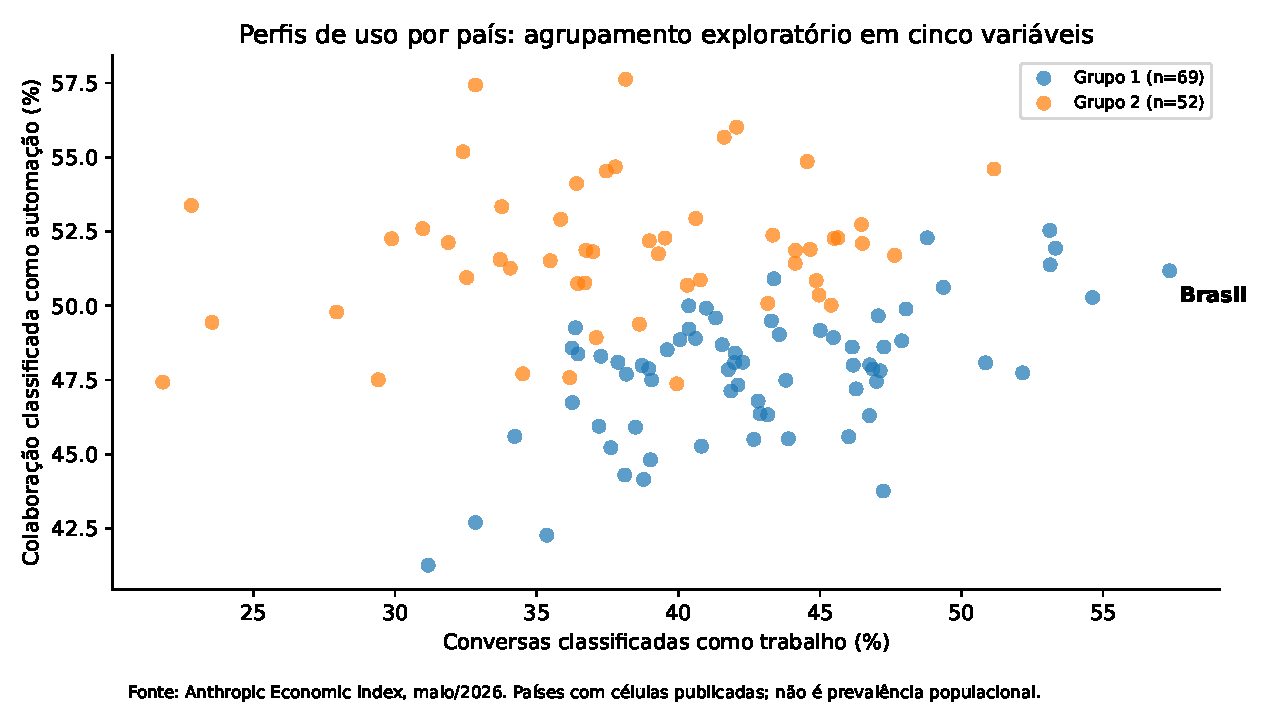
\includegraphics[width=\linewidth]{figures/countries.pdf}
\caption{Perfis nacionais de uso em maio de 2026. Cada ponto representa um país; as cores indicam os grupos de K-means calculados em cinco variáveis padronizadas. Os eixos mostram duas dessas variáveis em suas escalas originais: uso para trabalho e colaboração classificada como automação, em porcentagem. Fonte: análise própria dos agregados Anthropic.}
\label{fig:countries}
\end{figure}

Na Figura~\ref{fig:countries}, deslocar-se para a direita significa maior participação de conversas classificadas como trabalho; deslocar-se para cima significa maior proporção de colaboração classificada como automação. Cada país recebe um ponto de mesmo tamanho, independentemente de população ou volume de uso. As cores identificam os 69 países do grupo 1 e os 52 do grupo 2. A visualização utiliza duas coordenadas observadas, e não componentes de uma análise de componentes principais (PCA). Como o agrupamento considera também estudo formal, autonomia e escolaridade estimada da tarefa, pontos próximos nesse plano podem pertencer a grupos diferentes. A sobreposição é, portanto, compatível com a construção do modelo e com a separação limitada.

O Brasil aparece à direita da maior parte dos países, com 57,35\% de uso para trabalho, e em posição intermediária no eixo de automação, com 51,18\%. Essa combinação indica um perfil mais orientado a tarefas profissionais no recorte publicado, sem identificar o país de maior automação ou demonstrar dependência. O contraste entre as cores sugere diferenças de composição de uso; a comparação dos perfis em cinco dimensões e a estabilidade por subamostragem fornecem evidência mais completa do que a distância visual entre dois pontos.

No Brasil, a participação do uso publicado passa de 2,81\% em abril para 3,33\% em maio, e o índice per capita de 0,86 para 0,96. O último valor significa uso próximo, mas ainda inferior, ao proporcional à população em idade ativa na definição do índice. A colaboração classificada como automação cai ligeiramente de 51,51\% para 51,18\%. O país pertence ao grupo 1, mas não pode ser descrito como mais ou menos ``dependente'' com base nesses indicadores. O valor de agosto de 2025, 0,926, é uma referência adicional; diferenças de produto, janela e classificação impedem inferir uma trajetória mensal contínua.

Entre 120 países com informação econômica compatível, a associação descritiva de Spearman entre PIB por pessoa em idade ativa e índice de uso de maio é 0,931. Entre os 114 países presentes em abril e maio, a correlação das posições do índice é 0,996. A persistência das posições e a associação com renda podem refletir acesso, idioma, preços e seleção da plataforma. Além disso, PIB por pessoa e índice de uso envolvem normalização populacional, aspecto que pode contribuir para sua associação e exige cautela na interpretação. Não se isolaram esses mecanismos ou efeitos de normalização, nem se demonstrou que renda cause delegação problemática.

\subsection{Cruzamento GitHub--Anthropic: densidade digital e seleção}
A tabela GitHub dos dez maiores contingentes de contas possui oito correspondências com o recorte geográfico Anthropic. China e Rússia ficaram sem correspondência e não receberam valores presumidos. A correlação entre contas GitHub por mil pessoas em idade ativa e índice de uso Anthropic é 0,857 nesse conjunto selecionado. Os dois indicadores envolvem normalização populacional, os numeradores e denominadores têm datas distintas e contas não equivalem a pessoas únicas. O contingente GitHub também não está restrito à faixa etária do denominador. A razão construída descreve densidade relativa de contas; a correlação é exploratória e ecológica em oito casos, sem equivaler a estimativa mundial ou prevalência de adoção individual.

Para o Brasil, o GitHub reporta 10,2 milhões de contas em setembro de 2026. A combinação com a população em idade ativa do arquivo-base produz cerca de 69,44 contas por mil pessoas. A coexistência de forte presença em desenvolvimento e índice Anthropic de 0,96 sugere distinguir tamanho de comunidade digital de intensidade relativa de uso em um fornecedor. Não se pode atribuir aos mesmos indivíduos as atividades medidas nas duas plataformas.

\subsection{Grupos ocupacionais: o canal altera a leitura}
No recorte de maio de 2026, as participações publicadas para computação e matemática são 23,80\% no chat/Cowork e 28,17\% na API, razão de 1,184. No mesmo grupo, o indicador de colaboração classificada como automação corresponde a 63,90\% e 94,58\%, respectivamente; ele não compartilha o significado da participação ocupacional. Apoio administrativo apresenta 7,89\% e 11,92\%, e educação e biblioteca, 12,79\% e 6,16\%. Os 22 grupos SOC de nível 1 publicados somam 98,74\% no chat e 91,56\% na API. Não se redistribuiu a parcela complementar, cuja existência impede interpretar os números como composição renormalizada exclusivamente entre esses grupos.

\begin{figure}[htbp]
\centering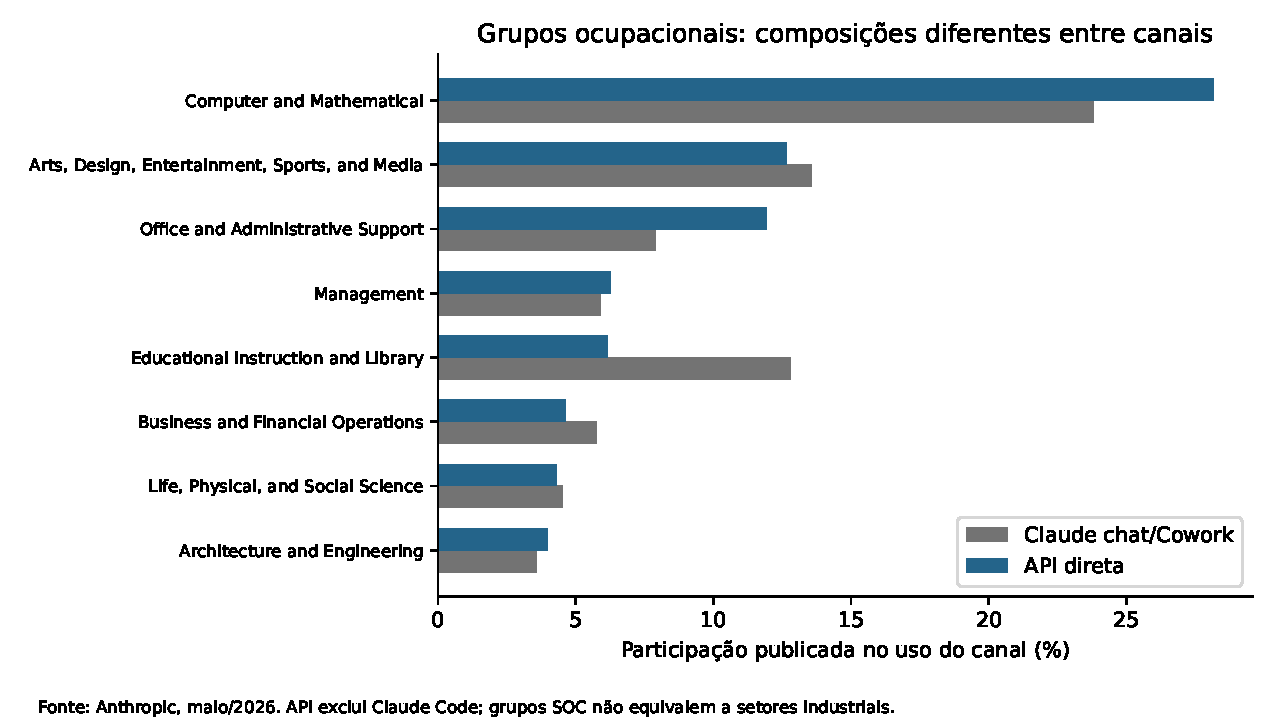
\includegraphics[width=\linewidth]{figures/occupations.pdf}
\caption{Composição ocupacional por canal em maio de 2026. São exibidos os oito grupos SOC com maior participação na API, ordenados pela participação nesse canal. Barras cinza representam chat/Cowork e barras azuis, API direta. O comprimento de cada barra indica a participação percentual nas tarefas classificadas do respectivo canal. Fonte: análise própria dos agregados Anthropic. A API exclui Claude Code.}
\label{fig:occupations}
\end{figure}

A leitura da Figura~\ref{fig:occupations} é horizontal: o eixo vertical identifica grupos ocupacionais, e o eixo horizontal mede sua participação publicada no uso de cada canal. Para uma mesma ocupação, a diferença entre as barras indica especialização relativa do canal. Computação e matemática têm a maior participação nos dois canais exibidos, com vantagem de 4,37 pontos percentuais na API; apoio administrativo apresenta diferença de 4,03 pontos a favor da API. Educação e biblioteca, por sua vez, têm participação 6,63 pontos maior no chat. O gráfico mostra, assim, perfis de demanda distintos, consistentes com interfaces e formas de integração diferentes.

Os oito grupos foram selecionados pela participação na API, e não por uma lista completa de setores ou pelo maior crescimento. Cada par de barras usa dois denominadores: 28,17\% na API e 23,80\% no chat não permitem concluir que a API tenha mais conversas de computação em termos absolutos. Os comprimentos representam participação ocupacional; os percentuais de automação de 94,58\% e 63,90\%, discutidos no texto, constituem outra métrica e não estão codificados nessas barras. Preservar essas distinções evita confundir composição de tarefas, quantidade de trabalhadores e intensidade de delegação.

O contraste ajuda a explicar por que um painel empresarial de APIs pode mostrar automação muito superior à observada em conversas de pessoas. Mudança de composição, ferramenta e interface é uma explicação concorrente ao suposto crescimento de dependência. Como o recorte de API exclui Claude Code, nem mesmo a categoria de computação representa todo o uso de agentes de programação. Tampouco se deve substituir a classificação ocupacional SOC pela industrial North American Industry Classification System (NAICS) usada no Octoverse.

\subsection{Tokens e gasto: sinais econômicos divergentes}
Nas 61 datas Vercel, considerando apenas laboratórios com cobertura completa, a média diária de participação de tokens de DeepSeek é 37,64\%, mas a de gasto é 4,95\%. Para Anthropic, os valores são 11,58\% e 39,30\%. A razão entre participação de gasto e de tokens é 0,132 no primeiro caso e 3,395 no segundo. Esse indicador é relativo à composição do gateway, não preço de tabela; médias diárias sem volumes absolutos não equivalem a participações acumuladas do período.

O relatório Vercel de outubro, referente a setembro, informa 71,5\% dos tokens e 23\% do gasto para modelos de pesos abertos \cite{verceloctober}. As médias relativas implícitas são $23/71{,}5=0{,}322$ para esse grupo e $77/28{,}5=2{,}702$ para o restante: uma razão aproximada de 8,40 sob o mesmo denominador e período. A composição inclui serviços e tarefas diferentes, não um ensaio de preço de modelos equivalentes. O relatório de novembro também registra modelos de decisão com cerca de 26\% das requisições e 0,53\% do gasto \cite{vercelnovember}. Requisições, tokens e despesa não fornecem rankings intercambiáveis.

Como apoio técnico, Bai et al. \cite{bai2026}, em preprint de 2026, analisam trajetórias de oito modelos em tarefas de programação agêntica e identificam elevada variabilidade de consumo, forte peso da entrada e ausência de correspondência simples entre mais tokens e maior acerto. A comparação pertence aos benchmarks e configurações examinados, não a toda equipe. O resultado reforça a necessidade de medir contexto reenviado, iterações e qualidade final, em vez de supor que saída longa seja a principal causa de custo.

\subsection{Previsão: o baseline vence e o teste final expõe instabilidade}
No backtest de 14 dias, a repetição sazonal de sete dias apresenta MAE de 5,04 pontos percentuais, seguida pelo Ridge com 5,72, tendência simples com 6,47 e persistência com 8,05. A escolha feita com essas janelas é mantida antes de observar o teste final. Nos cinco dias reservados, o baseline sazonal atinge MAE de 4,72, enquanto a persistência atinge 0,88 e o Ridge, 1,89. A ordenação muda entre janelas e horizontes diferentes; isso não isola uma causa para a mudança, mas impede sustentar superioridade preditiva estável do modelo de aprendizagem de máquina ou de um baseline único.

\begin{figure}[htbp]
\centering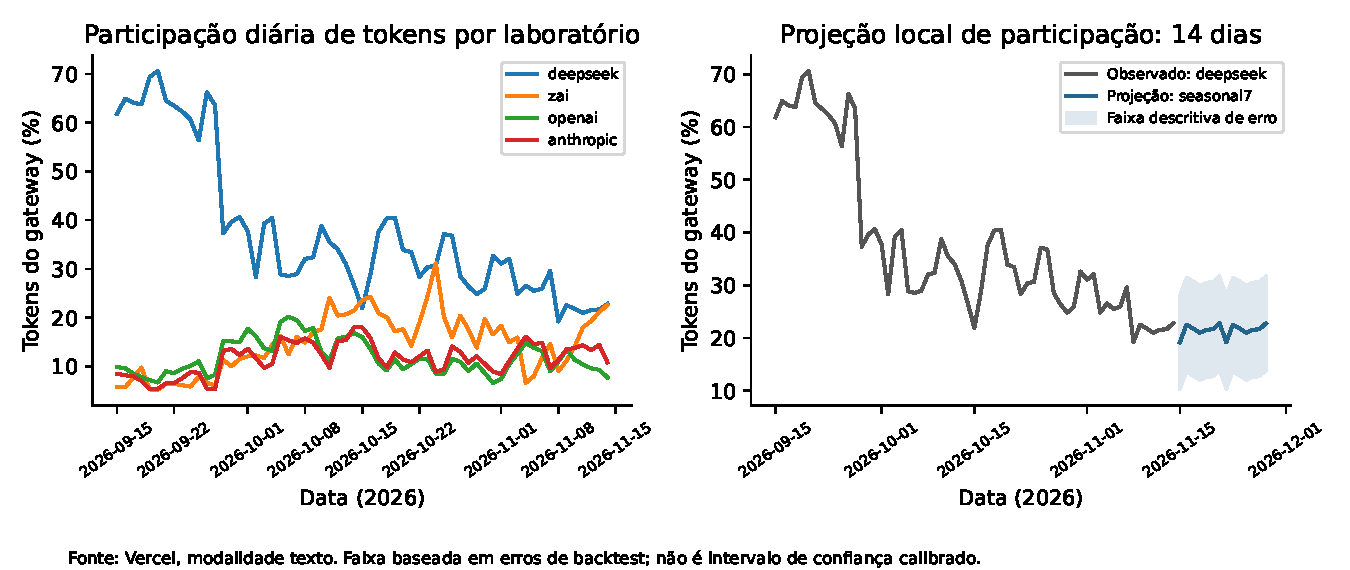
\includegraphics[width=\linewidth]{figures/gateway_forecast.pdf}
\caption{Participações de tokens e exercício de previsão na Vercel, modalidade texto. À esquerda, séries diárias dos quatro laboratórios de maior média com cobertura completa. À direita, a série observada de DeepSeek em cinza, a projeção de 14 dias por repetição sazonal de sete dias em azul e uma faixa descritiva de erro. As duas escalas verticais são percentuais dos tokens do gateway; não representam volume absoluto. Fonte: análise própria do snapshot Vercel.}
\label{fig:forecast}
\end{figure}

O painel esquerdo da Figura~\ref{fig:forecast} descreve a distribuição relativa dos tokens ao longo das 61 datas. Cada linha corresponde a um laboratório e cada ponto temporal, a sua parcela dos tokens de texto do gateway naquele dia. A redução da participação de DeepSeek ocorre enquanto outras séries ganham espaço relativo, mas o gráfico exibe apenas quatro laboratórios: as linhas mostradas não precisam somar 100\%. Uma participação em queda pode coexistir com crescimento do volume absoluto se o total do gateway aumentar. Sem os totais diários, não se quantifica demanda perdida ou crescimento mundial a partir dessas curvas.

No painel direito, a linha cinza reproduz a série de DeepSeek utilizada no experimento; a linha azul começa após a última observação e repete, por duas semanas, as participações dos sete dias anteriores. Seu formato periódico decorre da regra do baseline selecionado no backtest, sem demonstrar que um ciclo semanal persistirá. O sombreado corresponde à projeção acrescida e subtraída de aproximadamente 9,02 pontos percentuais, valor do percentil 90 dos erros absolutos de backtest, com limites em 0 e 100. Essa faixa não possui cobertura probabilística validada. A mudança do melhor método no teste final recomenda tratar a figura como exploração de sensibilidade de curto prazo, sem extrapolá-la para 2027 ou para consumo absoluto.

A extrapolação de 14 dias é divulgada como exercício de sensibilidade, não como ferramenta pronta para decisão de investimento. O horizonte curto, o teste final de apenas cinco dias e as janelas sobrepostas impedem uma avaliação robusta de incerteza. O achado metodológico é relevante: executar ML não obriga a preferi-lo, e apresentar sua limitação é parte do resultado científico.

\subsection{Cenários de insumos para 2027}
A Goldman Sachs divulga uma projeção de multiplicação de 24 vezes entre 2026 e 2030, alcançando 120 quadrilhões de tokens por mês \cite{goldman2026}. É previsão externa, não volume observado nem validação independente. Distribuir esse fator uniformemente por quatro anos produziria $24^{1/4}=2{,}213$ por ano. Essa interpolação constante é uma hipótese deste artigo, não uma previsão específica para 2027 atribuída à instituição.

Sob composição constante, um aumento de 50\% no volume com queda de 25\% no preço unitário gera fator de gasto $1{,}50\times0{,}75=1{,}125$, ou 12,5\% de aumento. Se o preço cair pela metade, o mesmo volume produz redução de 25\% no gasto. No cenário ilustrativo de fator 2,213, até uma redução de 50\% no preço implica aproximadamente 10,7\% de aumento no orçamento. Preço mais baixo, portanto, não garante fatura menor quando a quantidade aumenta.

Os cenários têm finalidade orçamentária e não projetam dependência. Não se converteram tokens diretamente em energia, água, GPUs ou emissões: arquitetura, modalidade, cache, utilização e matriz elétrica exigiriam coeficientes adicionais ausentes nas bases. No planejamento de equipes, a recomendação é acompanhar simultaneamente quantidade por tarefa validada, preço efetivo, latência, retrabalho e capacidade de revisão, em vez de um multiplicador global isolado.

\subsection{Pull requests e observabilidade: evidências e limites}
O Octoverse informa 110 milhões de PRs iniciados com rascunho de agentes em setembro de 2026, mais de 40\% do total, contra participação de 17\% em março; o volume aumentou aproximadamente seis vezes. Também reporta 1,3 bilhão de PRs mesclados e 34,3 bilhões de commits na janela anual \cite{github2026}. Crescimento de PRs não mede tokens, linhas úteis, qualidade ou perda de controle. PRs iniciados e PRs mesclados têm denominadores diferentes.

O mesmo relatório informa que, em setembro, aproximadamente 90\% dos PRs com agentes foram mesclados em duas semanas, comparados a cerca de 86\% dos demais. Essa observação não prova qualidade, mas impede tratar um gargalo universal de revisão como conclusão inevitável dos dados. A associação entre arquivo de configuração de agente e maior número de commits também não é efeito causal: projetos e equipes podem diferir em tamanho e atividade prévia.

Ferramentas como Langfuse e LiteLLM permitem organizar telemetria por chamada e custo \cite{langfuse2026,litellm2026}; a disponibilidade do software não torna públicos os dados de seus clientes. O anúncio Langfuse de 2026 sobre retirada de estimativas automáticas de tokenização ainda destaca que consumo ausente precisa permanecer visível. Telemetria incompleta não deve ser preenchida com falsa precisão. Sem uma série pública auditável de empresa, não é possível inferir sua evolução de tokens apenas por commits, tamanho de PR ou coautoria.

\section{Tokenaholics como proposta conceitual sociotécnica}
\subsection{Definição e fronteiras}
Propõe-se a seguinte definição de trabalho:
\begin{quote}
\textit{Tokenaholics designa, neste artigo, um padrão persistente de delegação à IA generativa em que dificuldades de regular o uso se articulam a enfraquecimento da verificação, da autonomia situada ou da capacidade de recuperação, com prejuízos relevantes ao trabalho, à aprendizagem ou à vida cotidiana.}
\end{quote}
A definição não está validada. ``Persistente'' exige investigação temporal; ``prejuízo relevante'' precisa ser documentado e contextualizado; ``autonomia situada'' significa capacidade de formular e avaliar decisões com os recursos legitimamente disponíveis. A expressão não pressupõe que autonomia seja fazer tudo sozinho. A colaboração humana, tecnologias assistivas e ferramentas de acessibilidade podem ampliar autonomia e devem ser preservadas na avaliação.

É útil distinguir dependência de infraestrutura, dependência funcional e uso problemático. A primeira ocorre quando um processo requer determinado serviço. A segunda descreve a distribuição de tarefas entre pessoa e ferramenta, que pode ser adequada. A terceira envolve dificuldade de regulação e consequências negativas. As três podem coexistir, mas não são equivalentes. Uma equipe que deixa de operar após queda de um serviço pode ter um problema de continuidade, ainda que seus integrantes mantenham competências e controle sobre o uso.

O termo tampouco deve funcionar como rótulo pessoal permanente. A unidade preferencial de análise é um padrão de prática em contexto: uma tarefa, uma equipe, um período e determinadas condições de acesso. A mesma pessoa pode utilizar IA de forma criteriosa em programação e de forma pouco regulada em outra atividade. Essa escolha reduz estigmatização e favorece intervenções verificáveis.

\subsection{Relação entre os achados agregados e a proposta}
Os achados delimitam o contexto em que uma hipótese de uso problemático precisaria ser investigada. Perfis nacionais diferentes podem decorrer de acesso, objetivos e seleção da plataforma; não distinguem pessoas que regulam adequadamente a assistência daquelas que experimentam prejuízo. A maior classificação de automação na API caracteriza um canal e suas tarefas, sem demonstrar enfraquecimento da autonomia de seus usuários. O contraste entre tokens e despesa mostra que volume e custo tampouco são substitutos suficientes de controle ou bem-estar.

A ausência de superioridade preditiva estável recomenda cautela em estimativas operacionais baseadas em séries curtas. Essa cautela não constitui evidência de compulsão. Para testar Tokenaholics seriam necessárias medidas de regulação, verificação, compreensão e consequências, acompanhadas longitudinalmente e contextualizadas nas condições de trabalho. As dimensões abaixo e a agenda futura especificam essa passagem do contexto agregado à investigação individual ou de equipe; não são variáveis observadas nos modelos aqui executados.

\subsection{Dimensões observáveis propostas}
Apresentam-se cinco dimensões para futuras pesquisas, sem pesos, limiares ou valor diagnóstico:
\begin{enumerate}
\item \textbf{Regulação do uso:} capacidade de encerrar consultas quando critérios de aceite são atendidos, respeitar objetivos próprios e explicar por que uma nova chamada é necessária.
\item \textbf{Verificação e contestação:} identificação de erros deliberadamente inseridos, busca de evidências independentes e disposição para rejeitar sugestões inadequadas.
\item \textbf{Compreensão e transferência:} capacidade de explicar a solução, adaptar princípios a um problema novo e distinguir código familiar de código apenas reconhecível.
\item \textbf{Recuperação e continuidade:} preservação de alternativas proporcionais à atividade quando o serviço falha, sem exigir domínio manual de toda a infraestrutura computacional.
\item \textbf{Consequências e contexto:} efeitos sobre prazos, retrabalho, aprendizagem e bem-estar, considerando metas, acessibilidade, apoio da equipe e liberdade de escolha.
\end{enumerate}
Essas dimensões deliberadamente permitem resultados divergentes. Um participante pode ter alto volume e boa regulação; outro, baixo volume e aceitação acrítica de uma decisão de alto impacto. Um instrumento que classificasse o primeiro como mais dependente apenas pelo consumo falharia em validade de construto.

\subsection{Um ciclo hipotético e suas alternativas}
O modelo proposto parte de uma situação de incerteza ou pressão. A pessoa delega parte da tarefa, recebe uma resposta e experimenta redução de esforço ou de insegurança. Se a resposta for incorporada sem verificação adequada e a entrega for recompensada apenas pela velocidade, novas delegações podem se tornar a resposta padrão. Com menos oportunidades de praticar avaliação, pode aumentar a dificuldade percebida de trabalhar em condições alternativas. Cada passagem é uma hipótese; o artigo não demonstra sua ocorrência causal.

O ciclo admite interrupções. Uma resposta pode ensinar um princípio e melhorar desempenho posterior. Uma equipe pode recompensar a detecção de falhas. Uma interface pode tornar evidências acessíveis. Um profissional experiente pode delegar deliberadamente a produção e concentrar esforço na revisão. Esses caminhos concorrentes tornam a proposta testável: se uso intenso preservar regulação, compreensão e desempenho, não há fundamento para classificá-lo como padrão problemático.

``Tolerância'' e ``abstinência'' não são adotadas como descritores estabelecidos. Preferir um modelo maior pode decorrer de tarefa mais difícil; precisar de mais contexto pode refletir projeto mais amplo. Para interpretar escalada, seria necessário comparar demandas equivalentes e investigar a finalidade das chamadas. A hipótese comportamental só ganha força quando explicações técnicas e organizacionais alternativas são consideradas.

\section{Implicações para sistemas, equipes e formação em computação}
\subsection{Arquiteturas que favoreçam controle e evidência}
As recomendações seguintes são propostas de engenharia derivadas da articulação conceitual; não constituem tratamentos nem tiveram sua eficácia demonstrada neste estudo. Uma aplicação pode apresentar orçamento por tarefa, número de chamadas e condição de encerramento. Agentes podem dispor de limite de iterações, escopo explícito e interrupção quando repetem uma falha. A finalidade é tornar o processo observável e controlável.

Propõe-se separar geração e aceite. Um artefato só deve ser considerado concluído após verificações adequadas ao risco: testes automatizados, análise estática, inspeção de dependências e revisão humana quando necessária. A avaliação deve ter alguma independência da geração. Pedir ao mesmo sistema que confirme sua resposta não oferece, por si só, essa independência. Casos de teste e documentação externa podem fornecer critérios adicionais, sem garantir ausência de erro.

Na interface, solicitações de justificativa podem ocorrer em decisões relevantes, evitando atrito em toda operação trivial. A pessoa pode registrar uma hipótese inicial, selecionar o que precisa ser verificado e comparar alternativas. Tornar cada clique difícil também pode aumentar frustração e prejudicar acessibilidade. O projeto deve avaliar o custo do mecanismo de controle e seus efeitos sobre diferentes usuários.

Minimização de contexto, recuperação seletiva e reutilização apropriada são possibilidades de eficiência. Sua adequação deve ser medida por tarefa e qualidade. Não se recomenda uma economia universal de tokens como objetivo independente: uma chamada adicional pode evitar uma falha grave. Também não se recomenda aumentar geração para demonstrar adesão à tecnologia. O orçamento é um limite operacional e uma oportunidade de reflexão, não um indicador de mérito.

\subsection{Aprendizagem e preservação de competência}
Bull e Kharrufa \cite{educacao} propõem integrar assistentes generativos à educação em desenvolvimento de software e discutem apoio gradual e redução desse apoio. Seu texto combina uma visão pedagógica com entrevistas exploratórias; não demonstra que um programa específico previna dependência. A contribuição ajuda a formular uma formação em que receber ajuda e aprender a avaliar essa ajuda sejam objetivos simultâneos.

Como desdobramento proposto, uma atividade pode alternar três momentos: formular uma solução inicial, usar a IA para explorar alternativas e resolver um problema de transferência com apoio reduzido. A avaliação deve observar explicação, testes e adaptação, além do produto final. As condições precisam ser compatíveis com tecnologias assistivas e com os objetivos da disciplina. O apoio não deve ser retirado de maneira punitiva ou sem justificativa pedagógica.

Em equipes, revisões de código podem perguntar que decisão foi delegada, qual evidência sustenta o aceite e o que permanece incerto. Essas perguntas documentam responsabilidade e ajudam a identificar lacunas de processo. Não se deve inferir incapacidade individual a partir de uma dificuldade pontual de explicação. A observação precisa considerar familiaridade com o domínio, tempo disponível e complexidade da alteração.

\subsection{Gestão e incentivos}
Assalaarachchi et al. \cite{gestao} analisaram 47 fontes de literatura cinzenta sobre IA generativa na gestão de projetos de software. A revisão registra possibilidades de apoio e preocupações com julgamento, privacidade e alucinações. Ela descreve discursos de profissionais disponíveis publicamente, sem representar todo o setor nem medir dependência. Sua inclusão amplia o foco para funções de coordenação, além da escrita de código.

Propõe-se que indicadores de produtividade combinem tempo, defeitos, retrabalho e capacidade de manutenção. Contagem de prompts, tokens ou linhas geradas não deve substituir resultados. Um ambiente que penaliza perguntas humanas e exige entregas imediatas pode incentivar delegação pouco examinada; essa relação deve ser investigada, em vez de atribuída automaticamente a características pessoais.

Uma política de continuidade também é pertinente: manter documentação de decisões, testes executáveis e alternativas de serviço para tarefas críticas. O objetivo é recuperar a operação e o entendimento quando uma ferramenta muda ou falha. Uma organização não precisa reproduzir manualmente um modelo de linguagem para preservar autonomia; precisa conhecer seus limites de dependência e as consequências de interrupções.

\section{Agenda empírica futura: validação ainda necessária}
\subsection{Perguntas e hipóteses refutáveis}
A primeira hipótese é que regulação e verificação expliquem consequências negativas melhor que volume bruto, após considerar dificuldade e experiência. A segunda é que uma interface com critérios de encerramento e evidências verificáveis reduza aceitação de erros em comparação com uma interface orientada apenas à geração. A terceira é que incentivos centrados exclusivamente em velocidade estejam associados a maior acúmulo de verificação pendente. Nenhuma dessas hipóteses foi testada neste manuscrito.

Uma hipótese alternativa é que usuários intensivos desenvolvam maior competência de supervisão e apresentem melhores resultados de transferência. Outra é que dificuldades de recuperação decorram principalmente da arquitetura e não da capacidade humana. Um estudo capaz de encontrar essas alternativas é mais informativo que um questionário concebido para confirmar que todo uso é dependência.

\subsection{Desenho misto e avaliação longitudinal}
Propõe-se acompanhar profissionais ou estudantes de computação em períodos sucessivos, com avaliação inicial de experiência, compreensão do domínio e familiaridade com ferramentas. O tamanho da amostra deve ser definido por análise de poder e viabilidade após especificação do efeito de interesse; não se oferece aqui um número arbitrário. Critérios de inclusão, desfechos e plano analítico deveriam ser registrados antes da coleta.

Um componente experimental poderia comparar interfaces e níveis de apoio em tarefas equivalentes, com distribuição aleatória e controle de ordem quando adequado. Erros inseridos para avaliar detecção deveriam ser confinados ao ambiente de pesquisa, com informação e esclarecimento ético apropriados. O resultado principal poderia ser a proporção de erros detectados, acompanhada de qualidade da solução, tempo, explicação e transferência posterior.

O componente longitudinal permitiria investigar mudanças dentro da mesma pessoa. Medidas repetidas ajudariam a separar familiaridade com a tarefa de possível perda de autonomia. A comparação com apoio reduzido deveria preservar recursos essenciais de acessibilidade. Desempenho sem uma ferramenta específica não deve ser tratado como medida universal de inteligência ou valor profissional.

Entrevistas e observação contextual examinariam por que cada consulta ocorreu, como o participante identifica conclusão suficiente e quais exigências organizacionais condicionam sua decisão. Esse componente é necessário para distinguir repetição improdutiva de exploração legítima e para interpretar o papel cultural da ferramenta. Resultados qualitativos não seriam convertidos automaticamente em prevalência populacional.

\subsection{Mensuração, privacidade e interpretação}
A telemetria mínima poderia registrar horário, contagem de chamadas, volume, duração e resultado de validação por tarefa. O conteúdo de prompts, código proprietário e dados pessoais não precisa ser coletado por padrão. Quando necessário ao objetivo científico, sua coleta exigiria justificativa, consentimento e proteção compatíveis. A pesquisa não deve transformar uma proposta de autonomia em mecanismo de vigilância laboral.

As análises deveriam considerar diferenças entre modelos, tokenizadores, tarifas e versões. Seria inadequado comparar contagens como se fossem unidades psicológicas equivalentes. Uma eventual escala exigiria estudo de conteúdo, entrevistas cognitivas, análise de estrutura, consistência e validade discriminante frente a intensidade de trabalho, confiança e experiência. Não se propõe um escore Tokenaholics pronto para aplicação.

Se uma intervenção reduzir tokens e simultaneamente piorar qualidade ou acessibilidade, não deve ser considerada bem-sucedida. Se aumentar consultas e melhorar verificação e aprendizagem, pode ser benéfica. O critério central é a qualidade da relação entre delegação, controle e consequência, com incerteza estatística explicitada quando houver dados.

\section{Limitações e responsabilidade conceitual}
A seleção dirigida do núcleo temático de doze obras e das dezessete referências complementares introduz viés de seleção e não representa consenso das áreas mobilizadas. A prioridade à computação e ao IEEE não substitui busca especializada em bases clínicas ou antropológicas. As bases empíricas têm seleção de plataforma, supressão de células e indicadores classificados ou estimados, sem amostra representativa do mercado mundial. O cruzamento GitHub--Anthropic contém oito países de uma tabela selecionada por tamanho da comunidade. Os numeradores GitHub são contas de usuários, sem restrição aos 15--64 anos do denominador populacional, reforçando que a razão construída não mede prevalência na população. O apoio psicológico da proposta provém sobretudo de uma revisão de escopo e de estudos de IHC, não de validação clínica própria.

Versões de repositório podem divergir das publicações finais. Arquivos e metadados foram confrontados, reduzindo risco bibliográfico sem assegurar ausência absoluta de erro; os preprints foram identificados como tais. Há análise secundária do Brasil, sem coleta primária ou amostra clínica nacional. Os métodos são exploratórios, sem pré-registro. O agrupamento não teve validação externa e sua estabilidade condiciona-se ao escalonamento mantido; o ARI não quantifica erros dos classificadores, arredondamento ou viés de cobertura. A curta série Vercel, as janelas sobrepostas, a seleção por cobertura na comparação descritiva e o teste final de cinco dias limitam a avaliação preditiva. A faixa apresentada não incorpora toda a incerteza de seleção, mudança de modelos ou comportamento futuro.

O termo proposto também pode reunir fenômenos excessivamente diversos. Se suas dimensões não apresentarem coerência ou utilidade além de conceitos existentes, a proposta deverá ser revisada ou abandonada. Há risco de estigmatizar uso assistivo, moralizar produtividade e transferir falhas organizacionais para indivíduos. Por isso, recomenda-se empregar o conceito para formular perguntas sobre práticas e sistemas, evitando classificar pessoas.

Por fim, ``silencioso'' não significa inevitável ou invisível a qualquer investigação. Significa apenas que uma entrega pode parecer satisfatória enquanto parte de sua verificação permanece pendente. Demonstrar que essa configuração é frequente, persistente e prejudicial exige estudos próprios. A formulação retórica do título não substitui essa demonstração.

\section{Considerações finais}
O estudo articula uma definição exploratória de Tokenaholics à caracterização do contexto sociotécnico de uso da IA generativa. A revisão fundamenta a distinção entre delegação, confiança excessiva e dependência; a análise secundária descreve perfis de países, diferenças ocupacionais entre canais e distribuições distintas de tokens e gasto. Nenhum desses indicadores mede diretamente regulação do uso, compreensão ou prejuízo funcional, e os achados não validam a existência, a prevalência ou as causas do padrão proposto.

A contribuição para a computação está no procedimento reproduzível de análise e no exame de limites de mensuração: agrupamentos apresentam separação limitada; participações ocupacionais preservam denominadores próprios; contas GitHub e uso Anthropic permitem apenas associação ecológica; e o melhor método de previsão muda entre backtest e teste final. Os cenários de 2027 mostram consequências condicionais de quantidade e preço com composição constante, sem estimar demanda mundial futura. Como implicação propositiva, recomenda-se avaliar tarefa validada, compreensão e recuperação junto ao custo, cuja utilidade para reduzir uso problemático ainda precisa ser testada.

Uma investigação responsável deve permitir que a proposta fracasse: usuários intensivos podem manter autonomia e obter benefícios; intervenções de restrição podem ser ineficazes ou prejudiciais. O compromisso científico é distinguir essas situações com evidências. O desafio colocado por Tokenaholics não é contar quanto uma pessoa conversa com a máquina, mas compreender se ela conserva condições de orientar, avaliar e interromper a delegação.

\noindent\textbf{Autoria da proposta conceitual:} Murillo Edson de Carvalho Souza apresenta neste manuscrito a definição de trabalho de Tokenaholics. Não se reivindica prioridade lexical mundial comprovada.

\medskip
\noindent\textbf{Disponibilidade e transparência:} código, entradas agregadas redistribuíveis, resultados, sementes, metadados e instruções constam da versão \texttt{v0.3.1} do projeto: \url{https://github.com/murilloed/tokenaholics-reproducible-study}. A reprodução confere os hashes de seis entradas, recalcula as análises e compara cinco sínteses com uma referência numérica fixa, usando tolerâncias explícitas. O ambiente e o commit são registrados por execução. O acesso ao repositório privado depende de autorização; a versão não possui DOI atribuído. Textos de terceiros permanecem no arquivo local de pesquisa, com links e direitos próprios. Não foram coletados dados de participantes. A preparação contou com assistência de IA generativa na pesquisa, organização e redação; o manuscrito permanece sujeito à revisão crítica e à aprovação do autor antes de submissão.

\bibliographystyle{IEEEtran}
\bibliography{reference}
\end{document}
